\section{Sequence Diagrams}

Sequence diagrams explain the chronological interaction among actors,
controllers, services, models, and infrastructure components. In the current
platform, the most important sequences are not limited to standard web CRUD
operations; they also include payment confirmation, virtual lab provisioning,
and controlled interaction with physical resources.

\subsection{Training Path Enrollment and Checkout Sequence}

This sequence begins when an engineer decides to access a paid or restricted
training path. The user selects the training path, initiates checkout, and is
redirected to the external payment flow when necessary. After Stripe confirms
payment through the webhook endpoint, the platform updates the payment state
and makes the related training path accessible through the learner's workspace.
The process can be summarized as follows:

\begin{enumerate}[topsep=0pt,itemsep=1pt,parsep=0pt,partopsep=0pt]
    \item Engineer selects a training path and initiates checkout
    \item Checkout controller creates the payment context
    \item External payment processor handles transaction validation
    \item Stripe webhook returns event data to the platform
    \item System validates the signature and records the webhook event
    \item Payment status is updated to completed or failed
    \item Enrollment access becomes available to the engineer
    \item The engineer can later consult payment history and request refund where
          applicable \end{enumerate} Figure~\ref{fig:seq-enrollment-checkout} illustrates the complete enrollment and checkout sequence, including the interaction between the frontend, the Laravel backend, and the Stripe payment processor.

\begin{figure}[H]
    \centering
    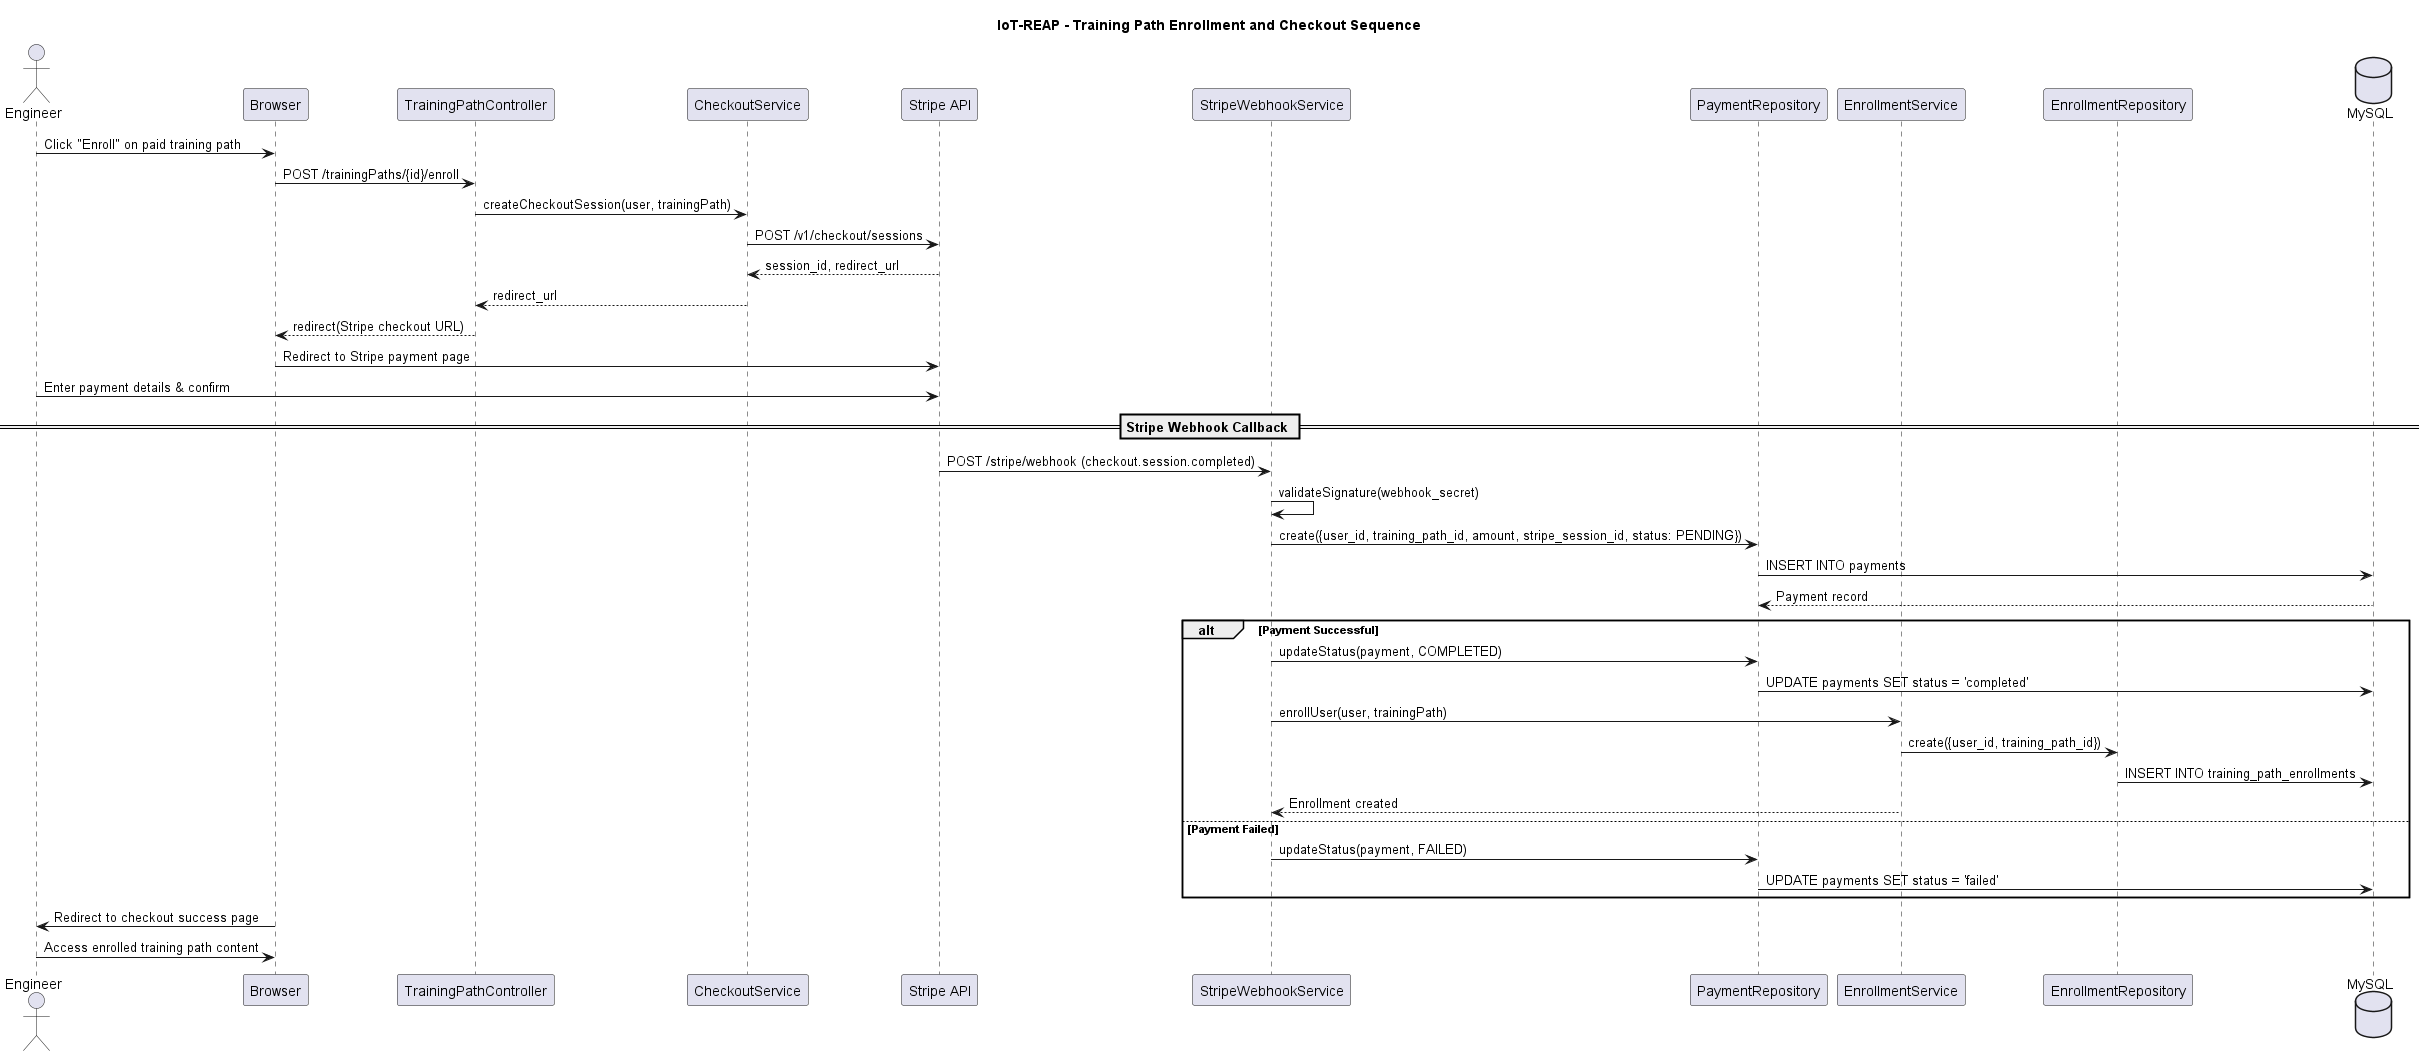
\includegraphics[width=0.95\textwidth]{assets/chapter3/iot-reap-sequence-enrollment-checkout.png}
    \caption{Sequence Diagram: Training Path Enrollment and Checkout}
    \label{fig:seq-enrollment-checkout}
\end{figure}

\subsection{Teacher Submission for Review Sequence}

This sequence models the transition from content authoring to publication
governance. A teacher edits the training path and associated learning units,
then submits the path for review. The platform validates ownership and
readiness, changes the review status, and exposes the path to the administrator
approval interface.

\begin{enumerate}[topsep=0pt,itemsep=1pt,parsep=0pt,partopsep=0pt]
    \item Teacher opens the teaching dashboard
    \item Teacher updates the training path structure and content
    \item Teacher triggers the submission action
    \item Controller validates role, ownership, and submission conditions
    \item Training path state changes to pending review
    \item Administrator later retrieves the submission from the administrative dashboard \end{enumerate} Figure~\ref{fig:seq-teacher-review} shows the teacher submission for review sequence, from content editing through the review status transition.

\begin{figure}[H]
    \centering
    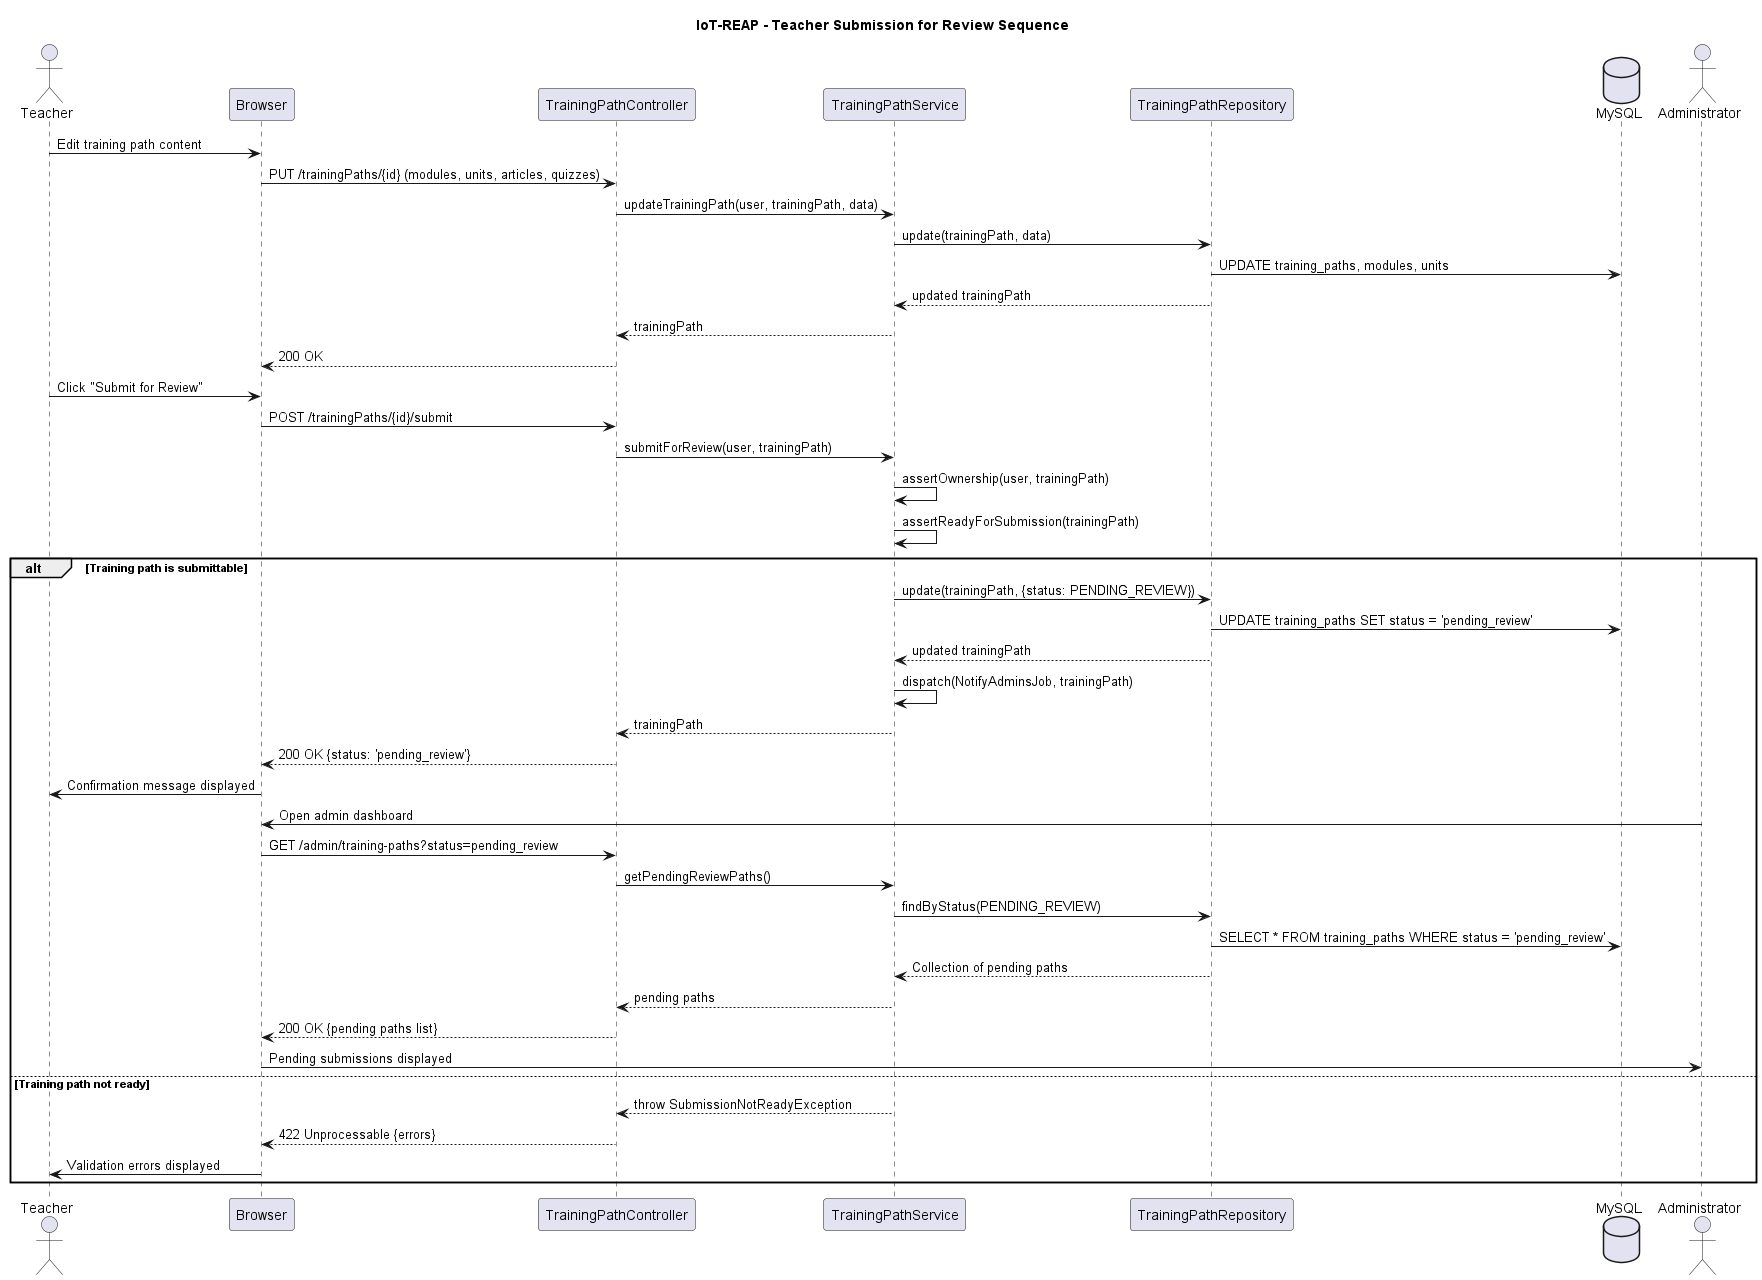
\includegraphics[width=0.95\textwidth]{assets/chapter3/iot-reap-sequence-teacher-review.png}
    \caption{Sequence Diagram: Teacher Submission for Review}
    \label{fig:seq-teacher-review}
\end{figure}

\subsection{Virtual Machine Provisioning Sequence}

The virtual machine provisioning sequence is a central differentiator of the
platform. It links the user interface to infrastructure models and remote
access capabilities.

\begin{enumerate}[topsep=0pt,itemsep=1pt,parsep=0pt,partopsep=0pt]
    \item Engineer sends a session creation request
    \item Session controller checks authentication, verification, and provisioning
          permission
    \item System evaluates available Proxmox servers and nodes
    \item A VM session is created and associated with infrastructure metadata
    \item The engineer consults the created session
    \item A Guacamole token is generated on demand for remote access
    \item The engineer may extend or terminate the session later
\end{enumerate}

Figure~\ref{fig:seq-vm-provisioning} presents the virtual machine provisioning
sequence, showing the interaction between the engineer, the session controller,
the Proxmox API, and the Guacamole remote access gateway.

\begin{figure}[H]
    \centering
    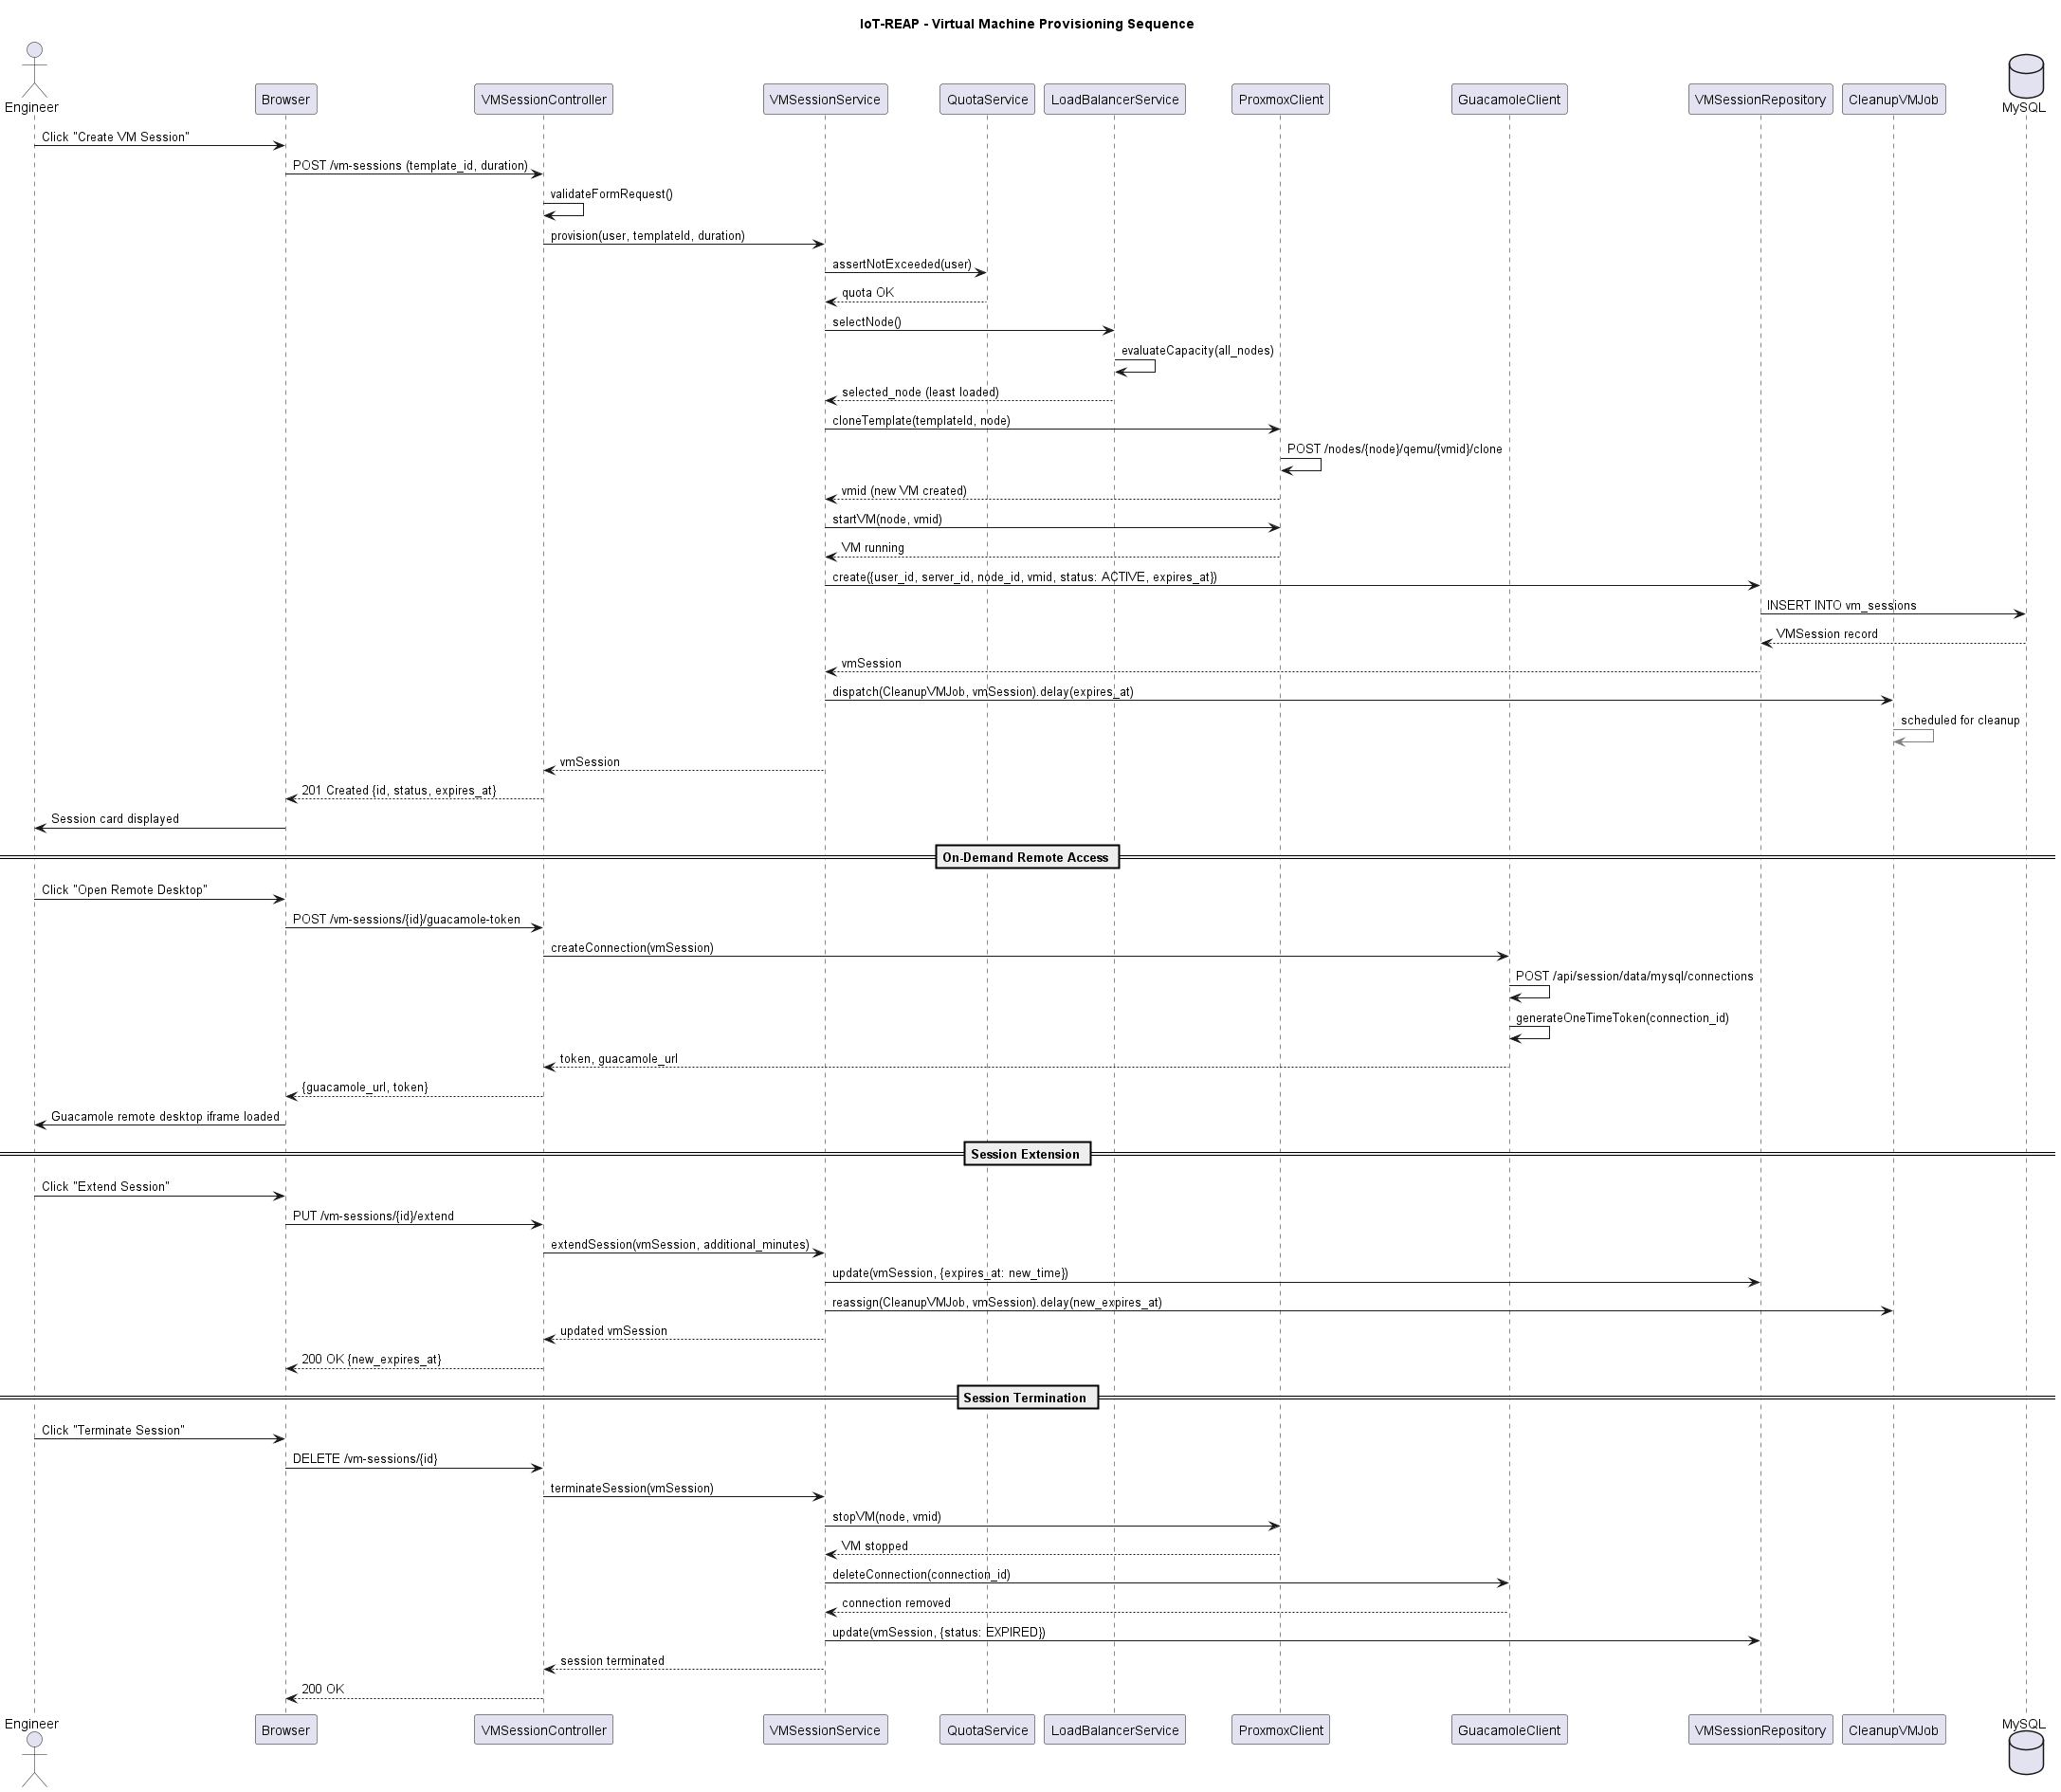
\includegraphics[width=0.95\textwidth]{assets/chapter3/iot-reap-sequence-vm-provisioning.png}
    \caption{Sequence Diagram: Virtual Machine Provisioning}
    \label{fig:seq-vm-provisioning}
\end{figure}

\subsection{Hardware Attachment and Queue Sequence}

This sequence governs access to USB devices attached to laboratory sessions.
Because some devices are exclusive or dedicated, the workflow includes queueing
behavior.

\begin{enumerate}[topsep=0pt,itemsep=1pt,parsep=0pt,partopsep=0pt]
    \item Engineer opens the hardware page associated with an active session
    \item System returns visible devices and their current state
    \item Engineer requests attachment of a selected device
    \item System checks whether the device is available, attached, reserved, or dedicated
    \item If the device is available, the attachment is executed
    \item If the device is busy, the engineer may join a waiting queue
    \item When the device becomes available, queue state is updated and notification can
          be issued
\end{enumerate}

Figure~\ref{fig:seq-hardware-attachment} illustrates the hardware attachment
and queue sequence, including the decision logic for device availability and
the waiting queue mechanism.

\begin{figure}[H]
    \centering
    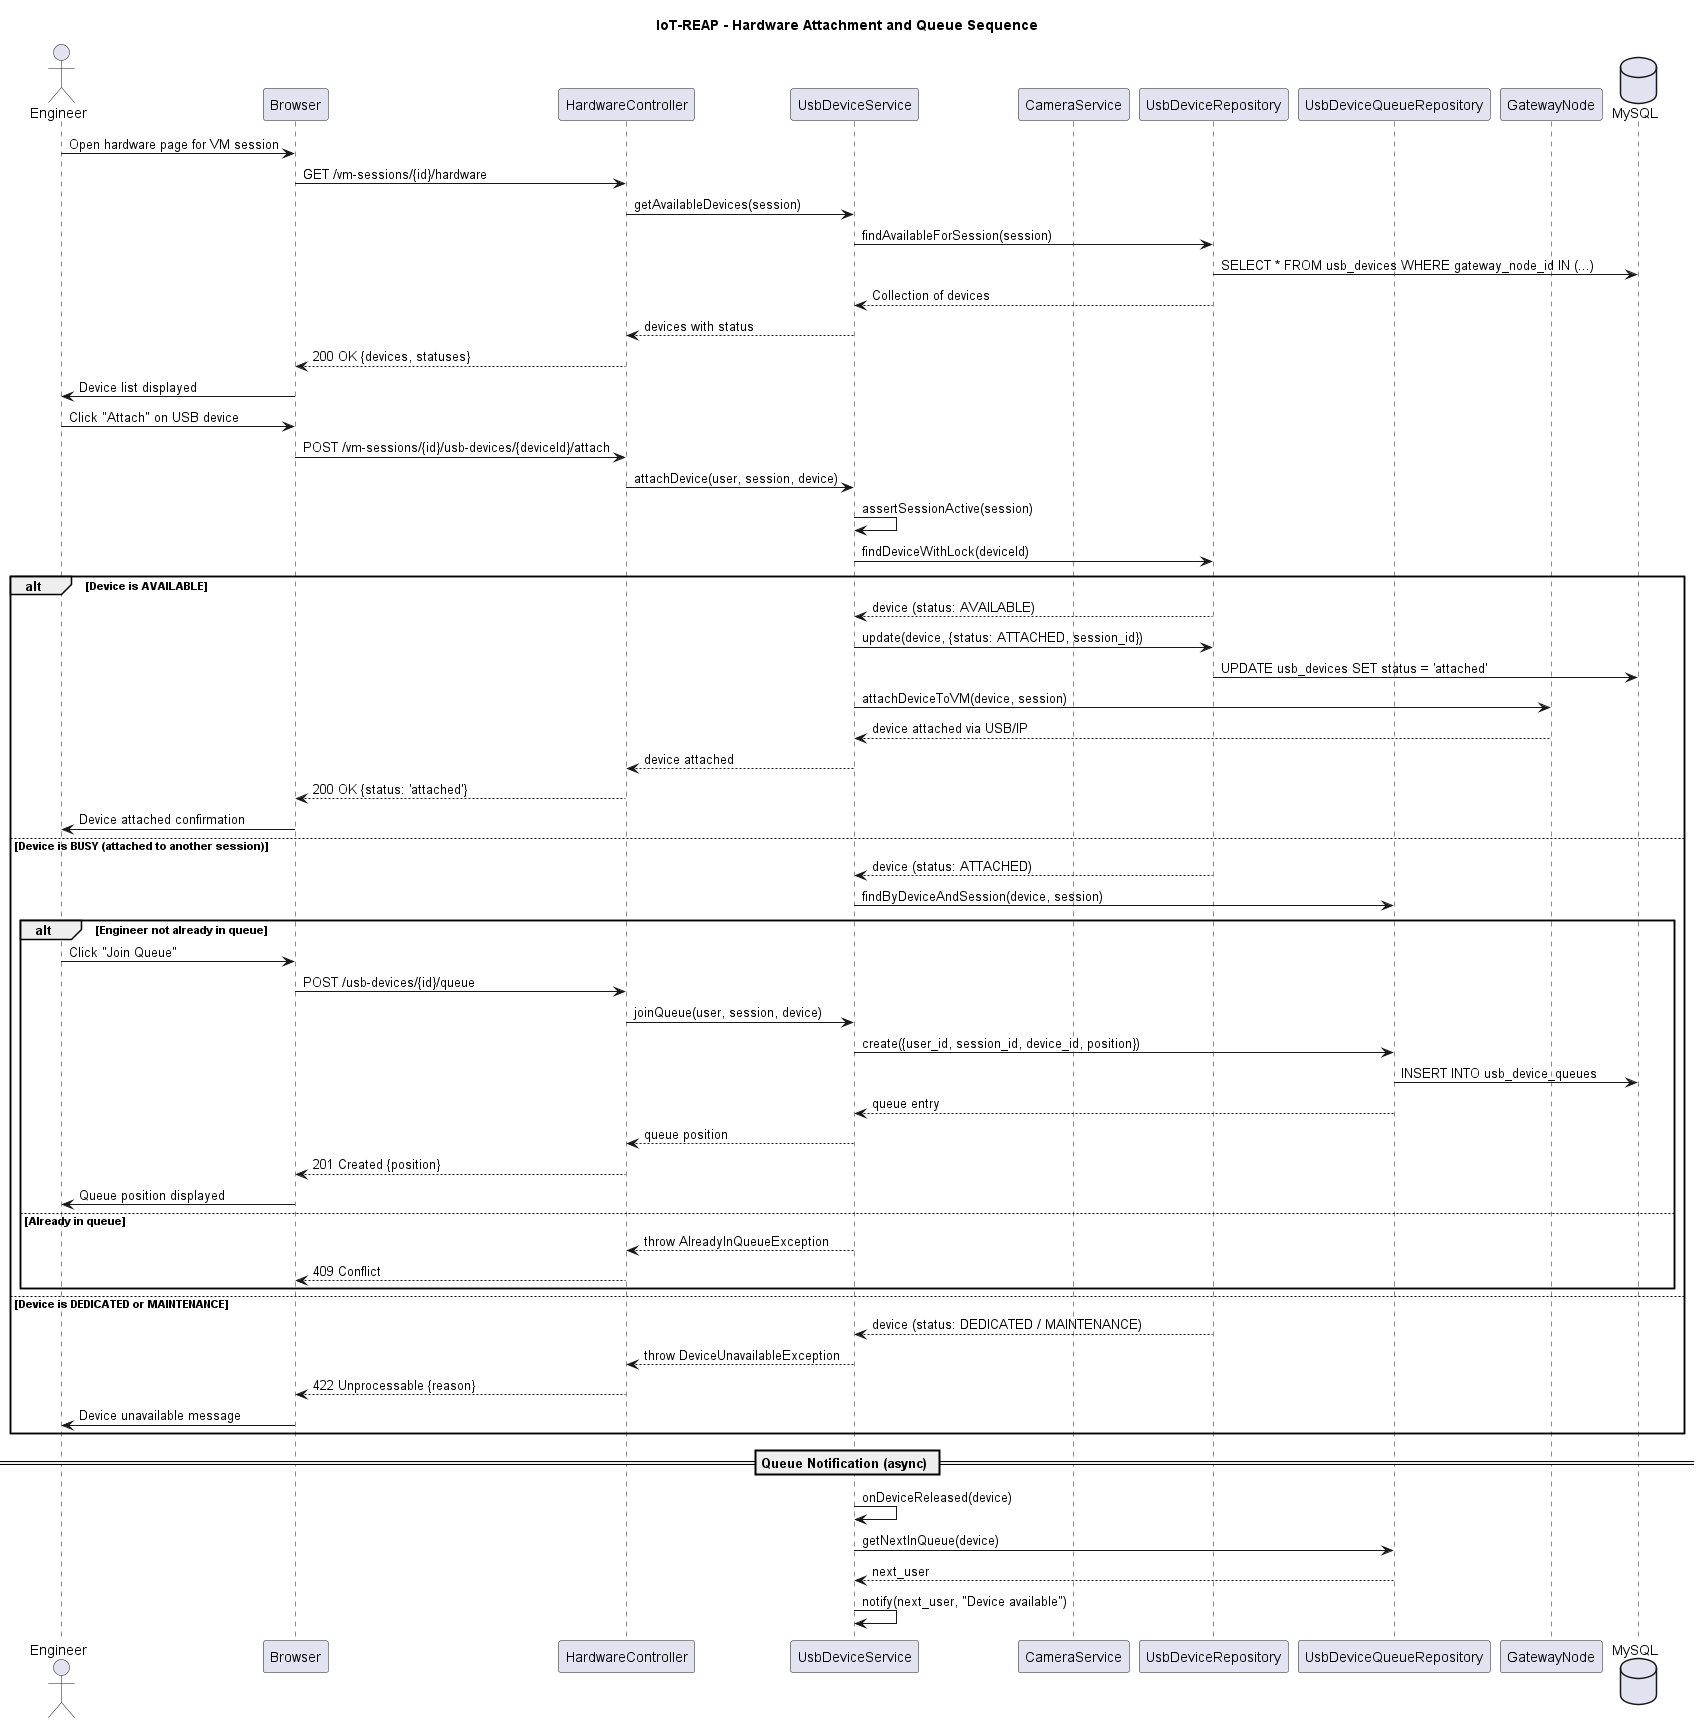
\includegraphics[width=0.95\textwidth]{assets/chapter3/iot-reap-sequence-hardware-attachment.png}
    \caption{Sequence Diagram: Hardware Attachment and Queue}
    \label{fig:seq-hardware-attachment}
\end{figure}

\subsection{Quiz Attempt Submission Sequence}

This sequence models the educational evaluation workflow.

\begin{enumerate}[topsep=0pt,itemsep=1pt,parsep=0pt,partopsep=0pt]
    \item Engineer opens the quiz associated with a training unit
    \item System verifies attempt eligibility
    \item A quiz attempt is created
    \item Engineer submits answers
    \item The platform validates and scores the attempt
    \item Attempt history and completion status are updated
    \item Training unit progress may be updated to reflect quiz completion or pass state
\end{enumerate}

Figure~\ref{fig:seq-quiz-attempt} shows the quiz attempt submission sequence,
from quiz opening through answer submission, scoring, and progress update.

\begin{figure}[H]
    \centering
    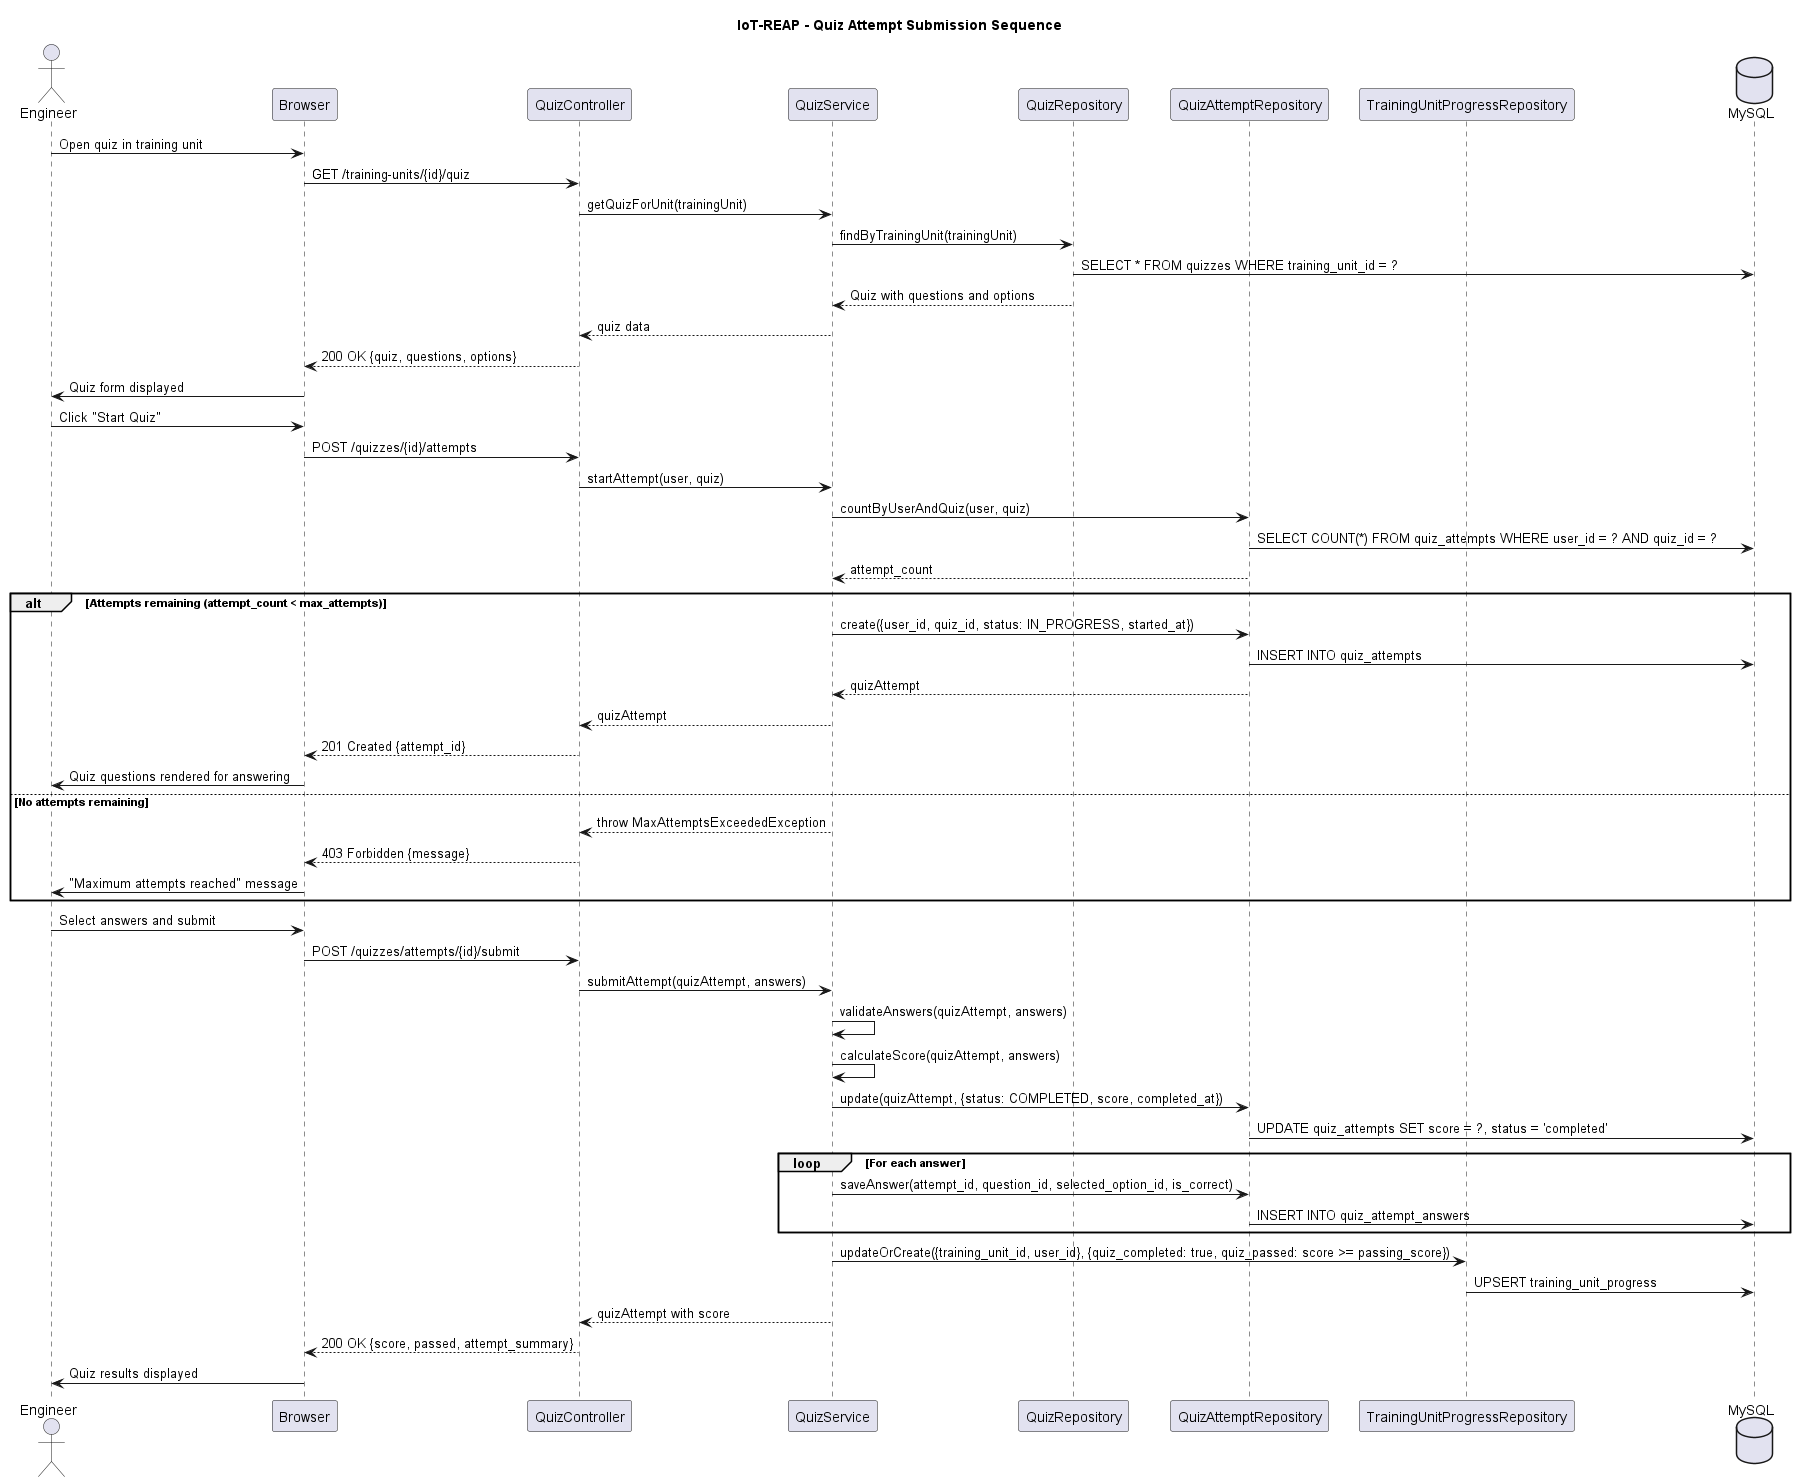
\includegraphics[width=0.95\textwidth]{assets/chapter3/iot-reap-sequence-quiz-attempt.png}
    \caption{Sequence Diagram: Quiz Attempt Submission}
    \label{fig:seq-quiz-attempt}
\end{figure}

\subsection{Google OAuth Authentication Sequence}

This sequence describes the social login flow when a user chooses to
authenticate through Google OAuth. The process leverages Laravel Socialite to
redirect the user to Google's consent screen, receive the authorization
callback, and either link the Google account to an existing user or create a
new account automatically. Role selection is presented when a new account is
created through this pathway.

\begin{enumerate}[topsep=0pt,itemsep=1pt,parsep=0pt,partopsep=0pt]
    \item Guest clicks the Google login button on the authentication page
    \item Laravel Socialite redirects the user to the Google OAuth consent screen
    \item User authenticates with Google and grants permission
    \item Google redirects back to the platform callback endpoint with an authorization
          code
    \item Socialite exchanges the code for an access token and retrieves user profile
          data
    \item System checks whether the Google account is already linked to an existing user
    \item If linked, the user is authenticated and redirected to their dashboard
    \item If not linked, a new account is created and the user is prompted to select a
          role
    \item User selects a role and the account is finalized with the chosen role
          assignment
\end{enumerate}

Figure~\ref{fig:seq-google-oauth} illustrates the Google OAuth authentication
sequence, showing the interaction between the user, the Laravel application,
and the Google identity provider.

\begin{figure}[H]
    \centering
    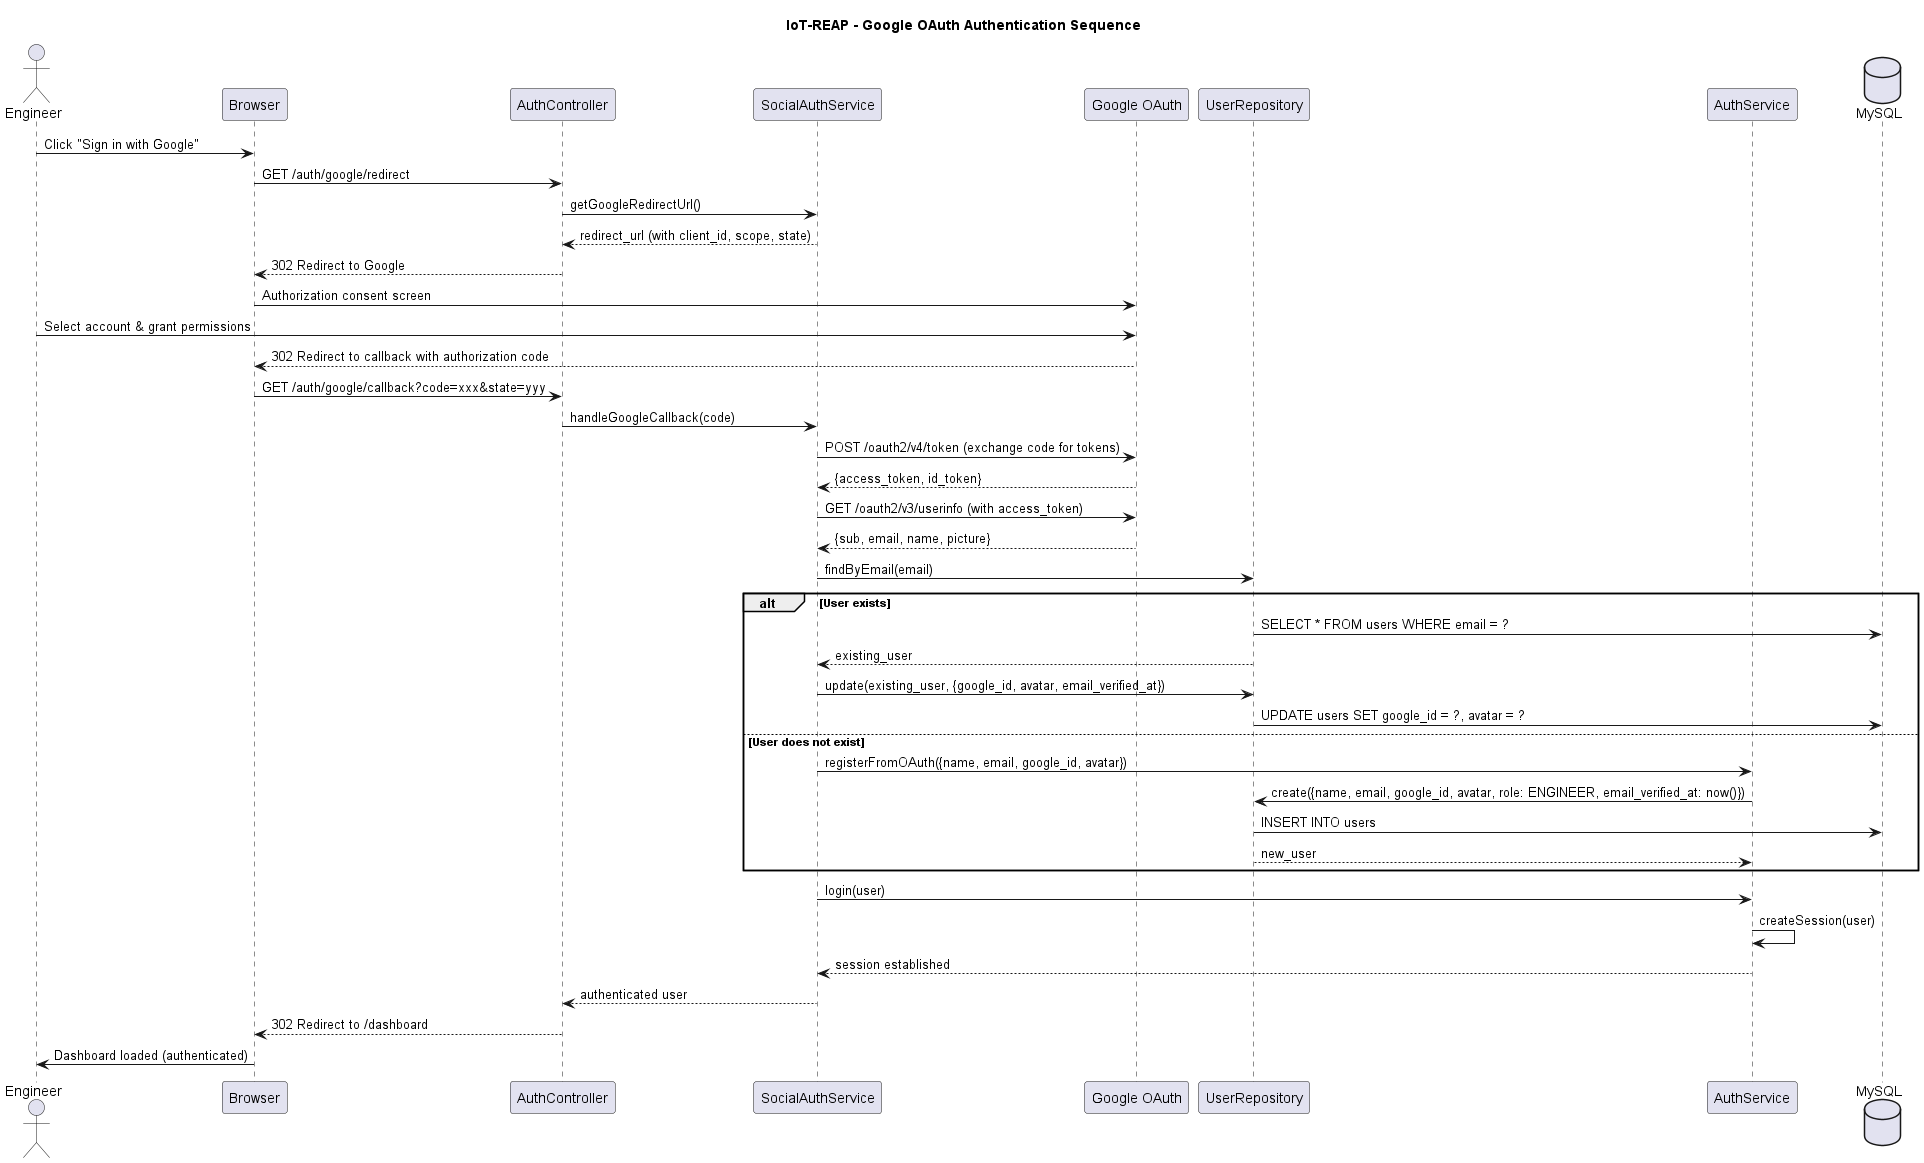
\includegraphics[width=0.95\textwidth]{assets/chapter3/iot-reap-sequence-google-oauth.png}
    \caption{Sequence Diagram: Google OAuth Authentication}
    \label{fig:seq-google-oauth}
\end{figure}

\subsection{MQTT Robot Control Sequence}

This sequence models the real-time command and telemetry exchange between an
engineer and a robot connected through the MQTT broker. The engineer issues
movement or action commands via the platform interface, which are published to
the robot's command topic. The robot executes the command and publishes
telemetry data back, which the platform subscribes to and relays to the
engineer's dashboard.

\begin{enumerate}[topsep=0pt,itemsep=1pt,parsep=0pt,partopsep=0pt]
    \item Engineer opens the robot control interface within an active VM session
    \item System verifies session ownership and robot access authorization
    \item Engineer issues a command through the control interface
    \item Platform publishes the command to the MQTT topic
          \texttt{robot/\{robot\_id\}/commands} with QoS 1
    \item Mosquitto broker delivers the command to the subscribed ESP32 controller
    \item Robot executes the command and publishes telemetry to
          \texttt{robot/\{robot\_id\}/telemetry}
    \item Platform MQTT subscriber receives the telemetry update
    \item Telemetry data is relayed to the engineer's interface through WebSocket or
          polling
    \item Engineer observes the updated robot state and may issue further commands
\end{enumerate}

Figure~\ref{fig:seq-mqtt-robot} presents the MQTT robot control sequence,
showing the publish-subscribe interaction between the engineer, the Laravel
backend, the Mosquitto broker, and the ESP32-controlled robot.

\begin{figure}[H]
    \centering
    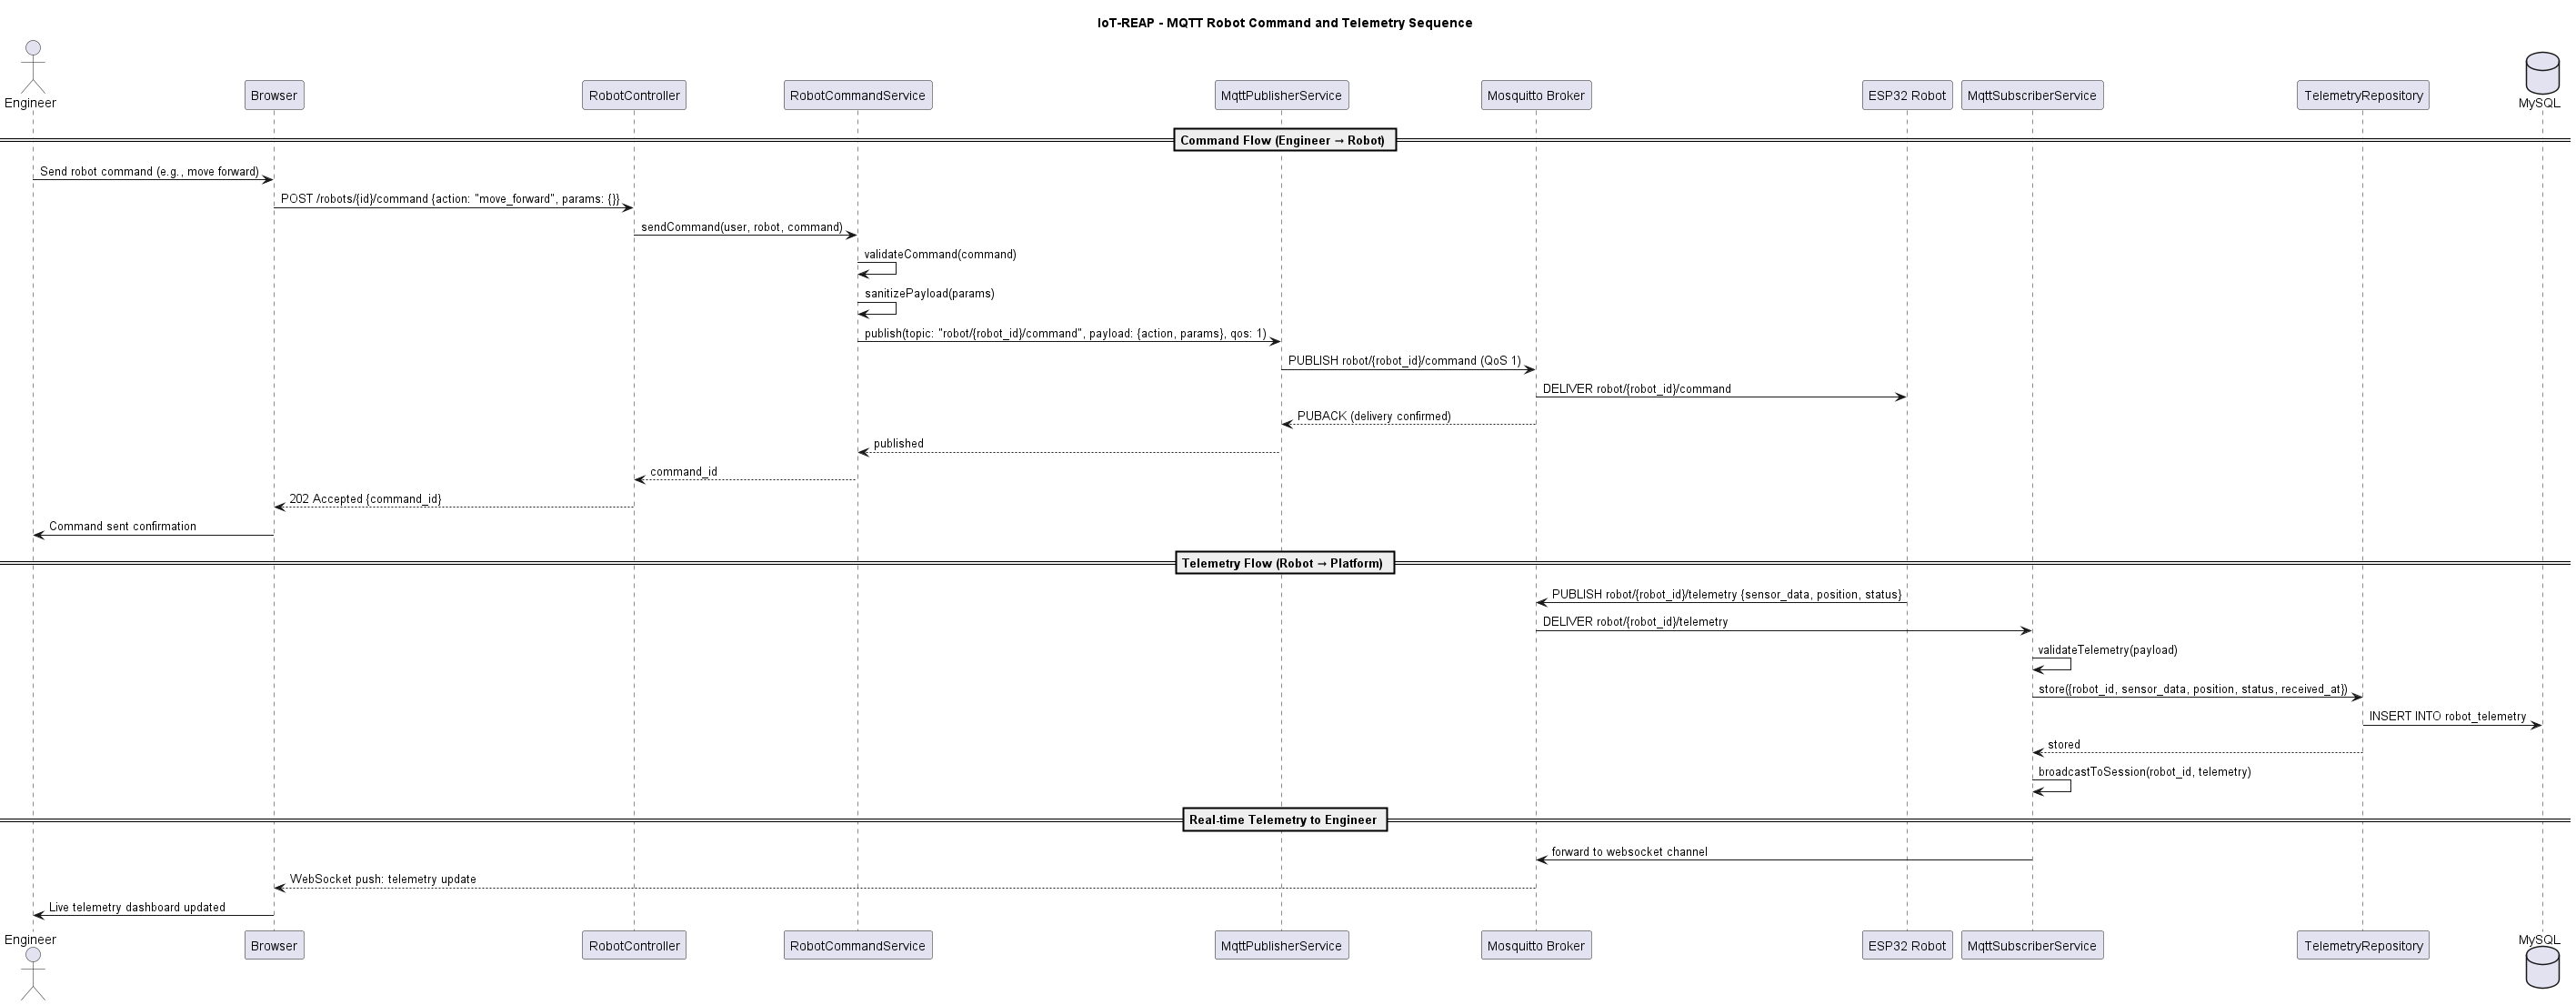
\includegraphics[width=0.95\textwidth]{assets/chapter3/iot-reap-sequence-mqtt-robot.png}
    \caption{Sequence Diagram: MQTT Robot Control}
    \label{fig:seq-mqtt-robot}
\end{figure}

\subsection{Camera PTZ Control Sequence}

This sequence describes how an engineer requests and exercises pan-tilt-zoom
control over a PTZ-enabled camera within an active VM session. The workflow
includes control request arbitration, exclusive session control creation,
movement command dispatch, and control release when the engineer finishes or
the session ends.

\begin{enumerate}[topsep=0pt,itemsep=1pt,parsep=0pt,partopsep=0pt]
    \item Engineer opens the camera stream view within an active session
    \item System displays the live camera feed and available PTZ controls
    \item Engineer requests camera control
    \item System checks whether the camera is currently controlled by another user
    \item If available, a CameraSessionControl record is created granting exclusive
          control
    \item Engineer issues PTZ movement commands through the interface
    \item System translates each command into camera-specific movement parameters
    \item Camera executes the movement and the updated frame is reflected in the stream
    \item Engineer may change stream resolution during the session
    \item When the engineer releases control or the session ends, the control record is
          removed
\end{enumerate}

Figure~\ref{fig:seq-camera-ptz} illustrates the camera PTZ control sequence,
from control acquisition through movement commands to control release.

\begin{figure}[H]
    \centering
    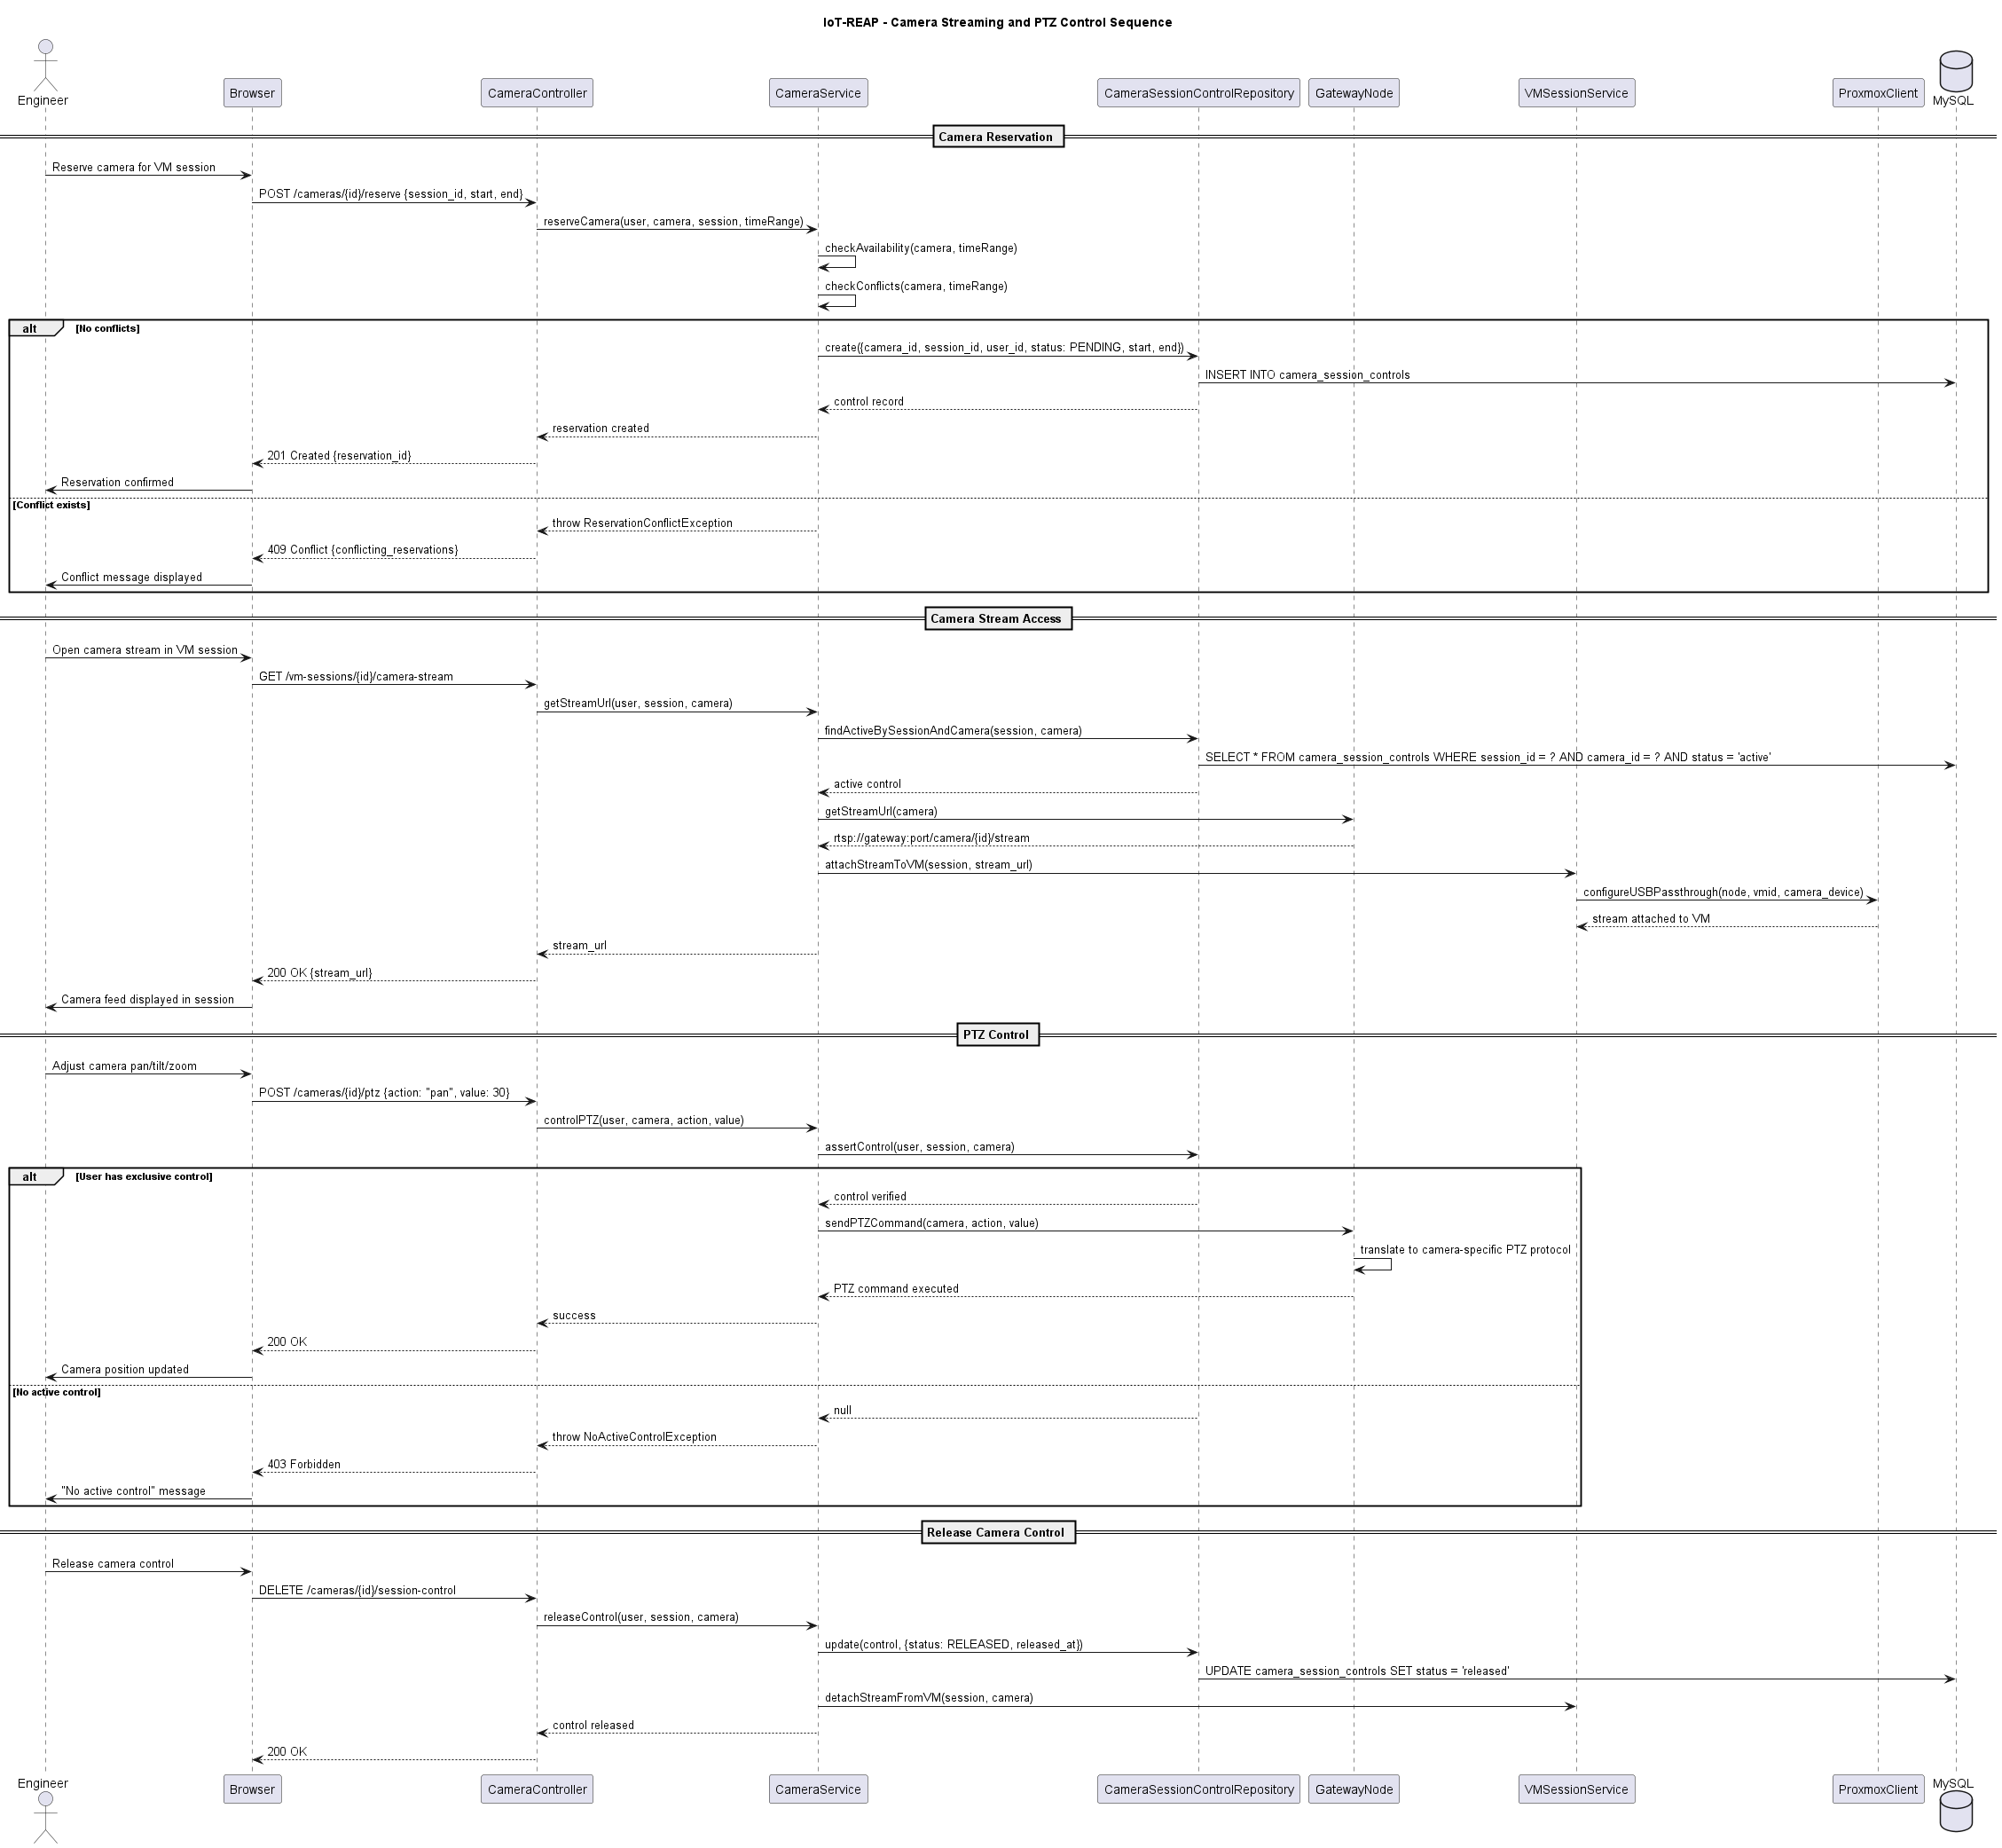
\includegraphics[width=0.95\textwidth]{assets/chapter3/iot-reap-sequence-camera-ptz.png}
    \caption{Sequence Diagram: Camera PTZ Control}
    \label{fig:seq-camera-ptz}
\end{figure}

\subsection{Refund Processing Sequence}

This sequence models the refund workflow from the engineer's initial request
through administrative review and potential Stripe refund execution. It
demonstrates how payment governance is handled as a multi-step auditable
process rather than a simple transaction reversal.

\begin{enumerate}[topsep=0pt,itemsep=1pt,parsep=0pt,partopsep=0pt]
    \item Engineer submits a refund request for a completed payment
    \item System validates that the payment exists and belongs to the requesting user
    \item A RefundRequest record is created with pending status
    \item Administrator opens the refund review interface
    \item Administrator reviews the payment context and refund reason
    \item Administrator approves or rejects the refund request
    \item If approved, the system initiates a refund through the Stripe API
    \item Stripe processes the refund and returns the result
    \item System updates the refund request status and the payment state accordingly
    \item Engineer is notified of the refund decision and outcome
\end{enumerate}

Figure~\ref{fig:seq-refund} presents the refund processing sequence, showing
the interaction between the engineer, the administrator, the Laravel backend,
and the Stripe refund API.

\begin{figure}[H]
    \centering
    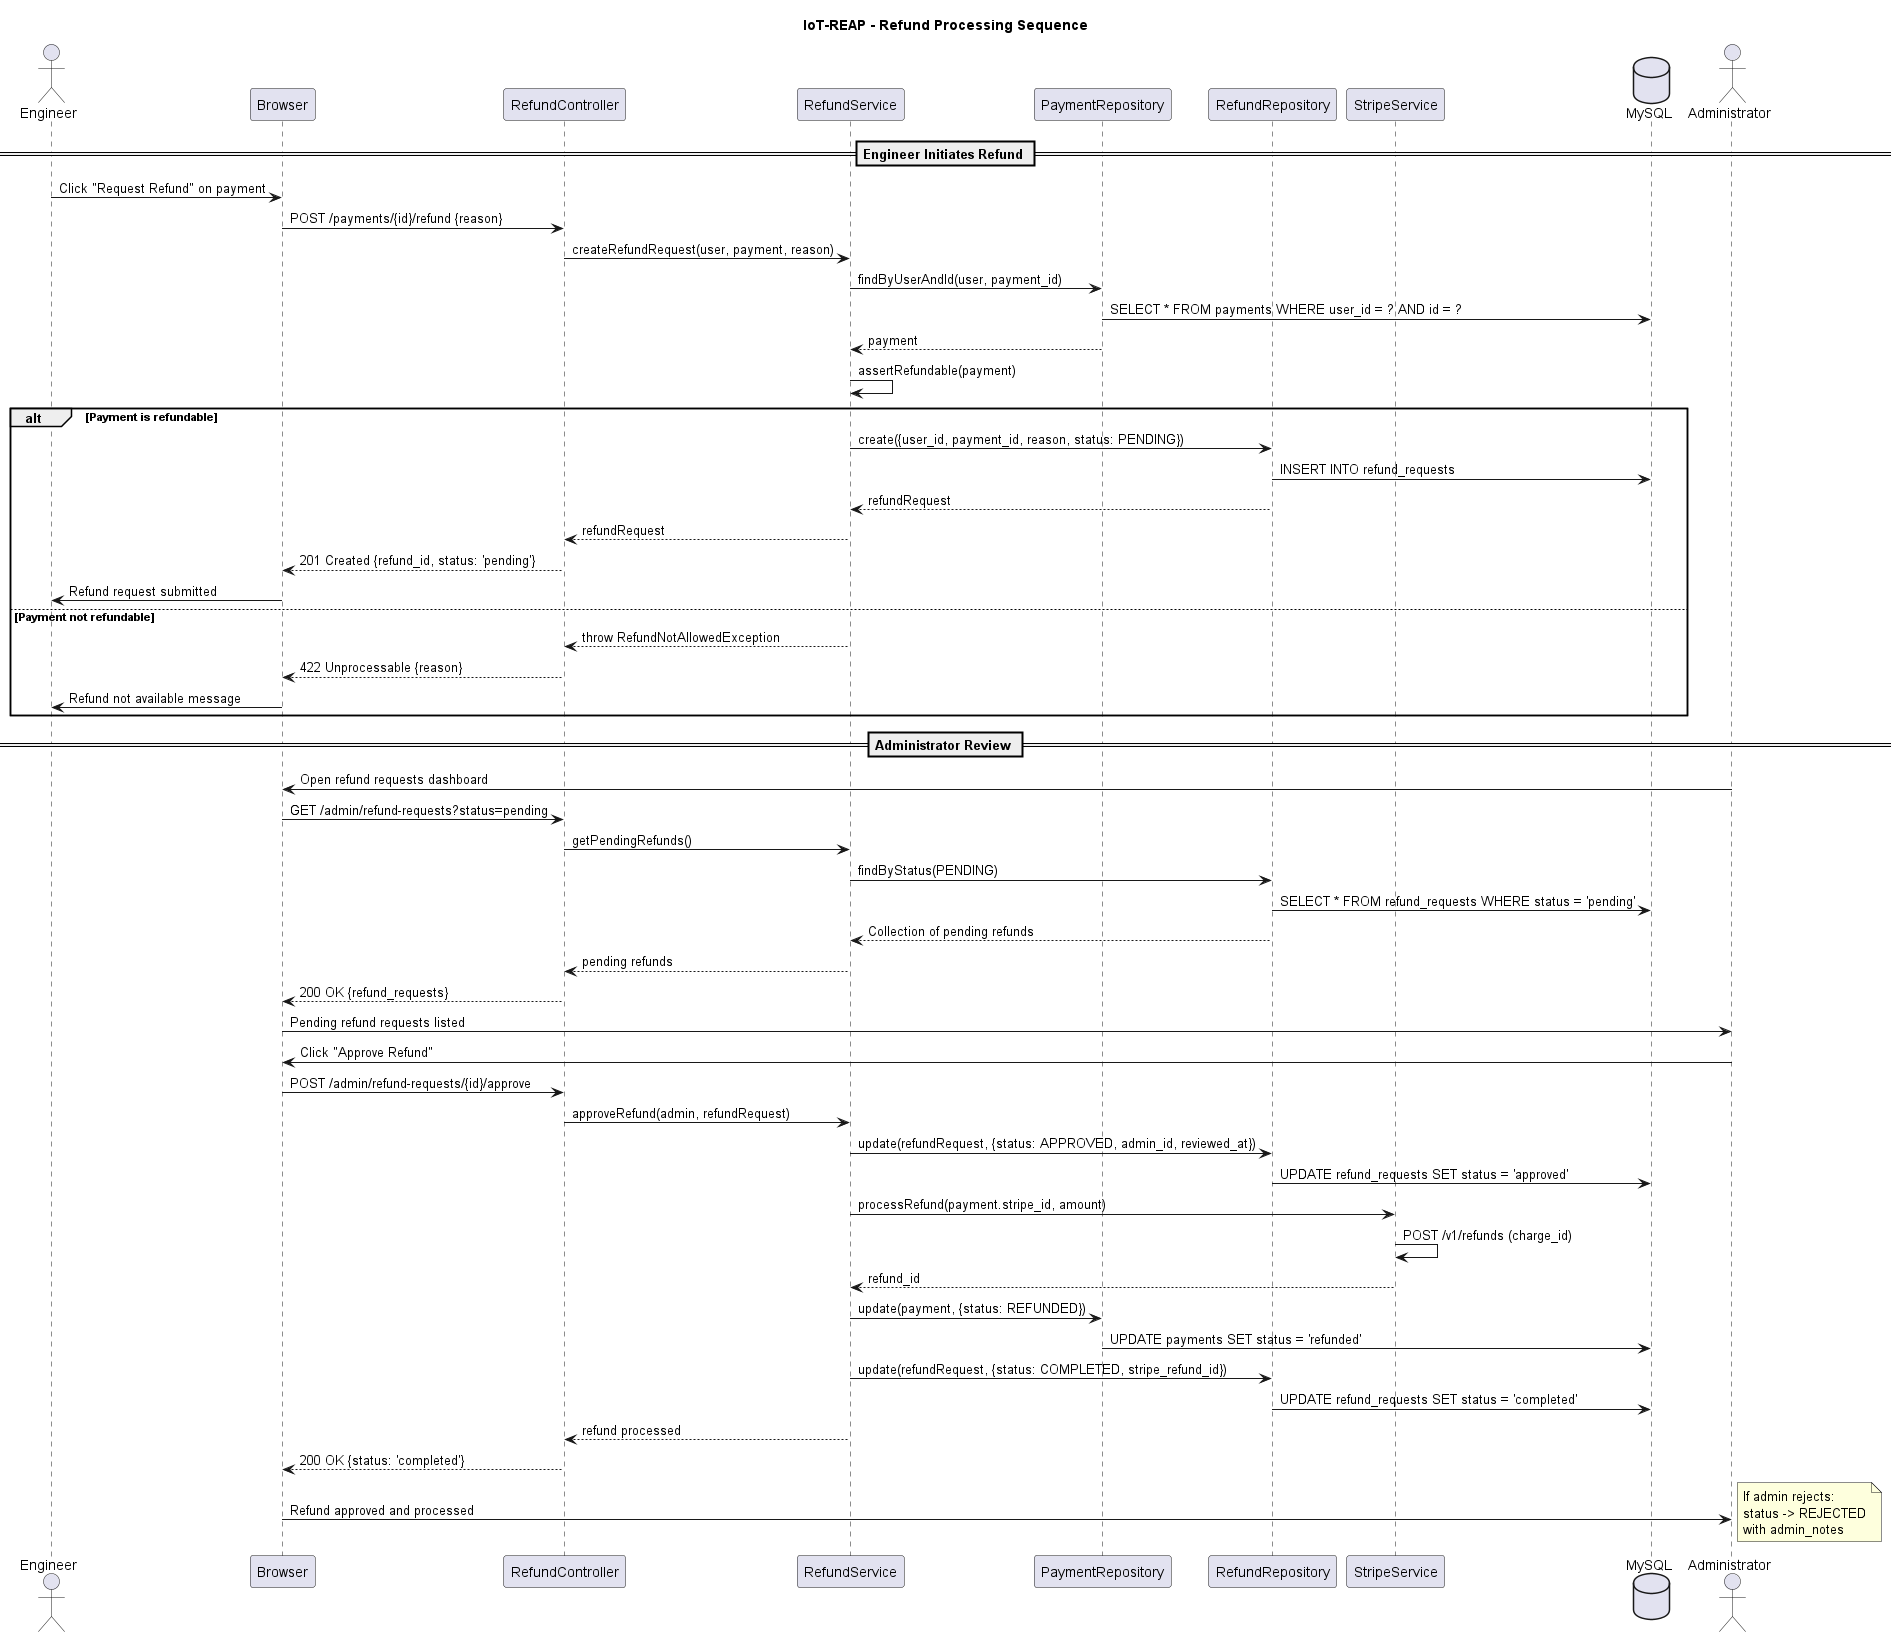
\includegraphics[width=0.95\textwidth]{assets/chapter3/iot-reap-sequence-refund.png}
    \caption{Sequence Diagram: Refund Processing}
    \label{fig:seq-refund}
\end{figure}
